\chapter{Results and Discussion}
The device has been designed completely from scratch. So to make it standard compliant it is necessary to test it's all aspect and keep them well below the limit so that final results are well within the stipulated guideline. Hence, here qualitative and quantitative results are presented which include computation latency, reporting rate \& variation, ADC response(s) and amplitude \& frequency estimation.

\subsubsection{Computation delay}
The following graph show the delay distribution of DFT computation, left hand side of plot shows normal operation while right hand side of the plot shows a loaded system performance. The "on-load" condition wont occur in real-life scenario but this was done just to evaluate overall capability and performance.
\begin{figure}[h]
	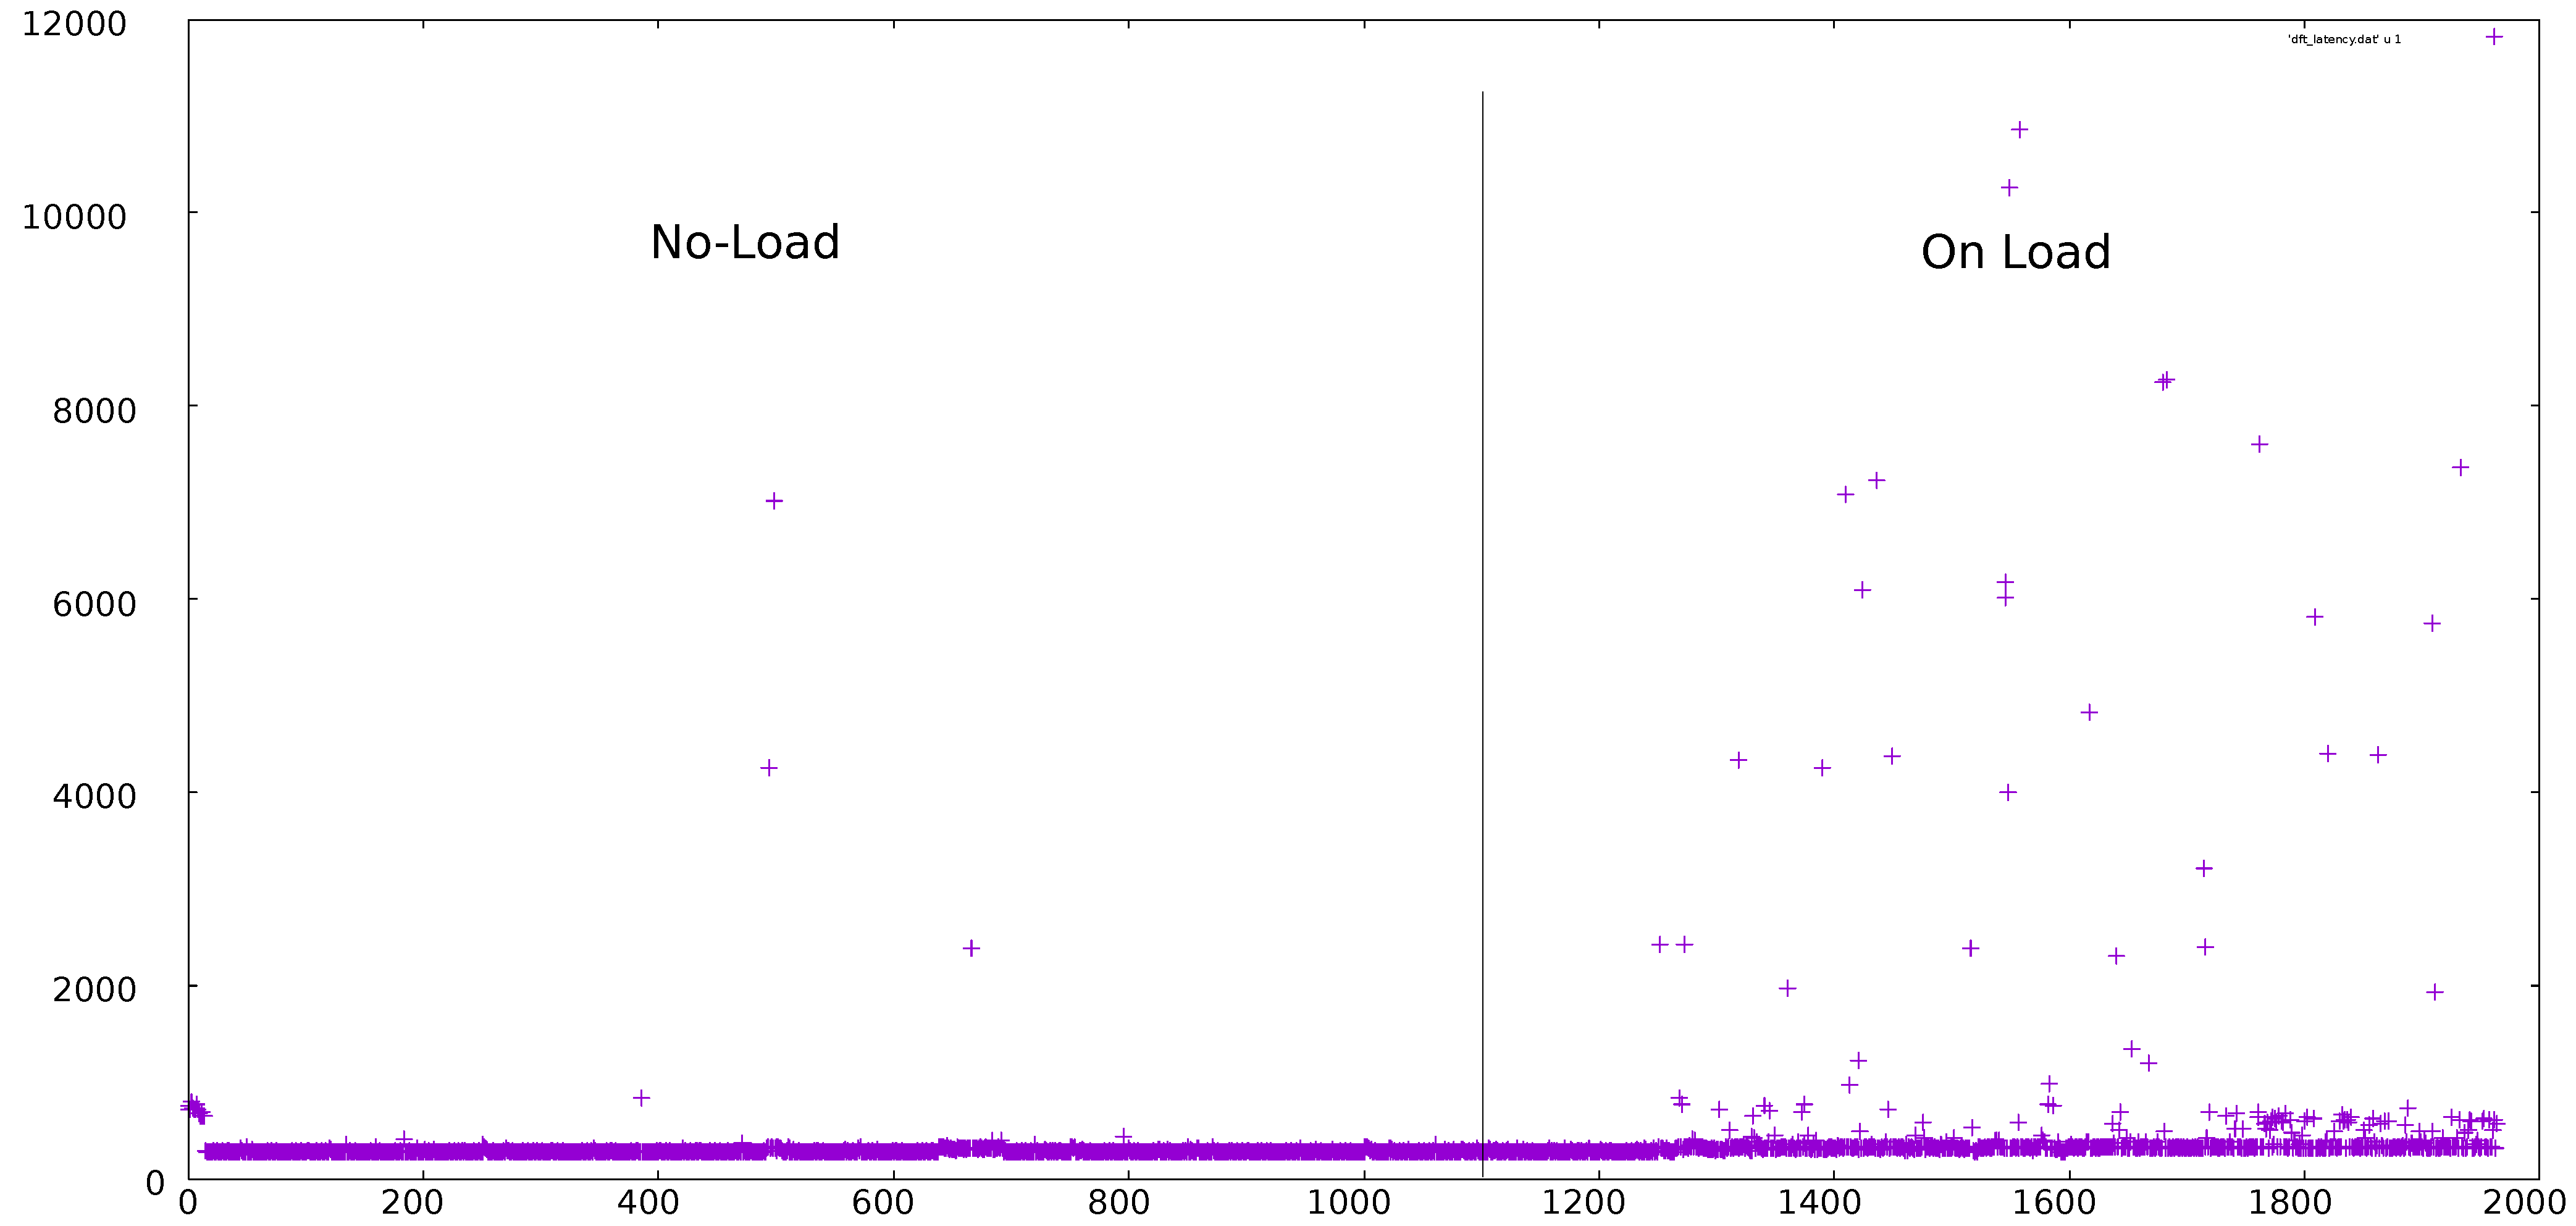
\includegraphics[scale=0.23]{fig/delay_test.eps}
\end{figure}
